\documentclass[aspectratio=43]{beamer}

\usepackage[T1]{fontenc}
\usepackage[utf8]{inputenc}
\usepackage[english]{babel}
\usepackage{pgfplots}
\pgfplotsset{compat=newest}
\usepackage{booktabs}
\usepackage{siunitx}

% Latin Modern
%\usepackage{lmodern}
% Verdana font type
%\usepackage{verdana}
% Helvetica
%\usepackage{helvet}
% Times (text and math)
%\usepackage{newtx, newtxmath}
% Nice font combination
\usepackage{mathptmx} % math
\usepackage{sourcesanspro} % sans-serif
\usepackage{charter} % serif

\usetheme[department=miljo]{DTU}

\title[DTU Templates]{DTU Beamer Template}
\author{Remus M. Prunescu}
\institute{\LaTeX\ Support Group, Technical University of Denmark (DTU)}
\date{\today}
	
\newcommand{\tabitem}{{\color{dtured}$\bullet$} }

\begin{document}
\frame{
	\maketitle
}

\frame{
	\frametitle{Outline}
	\tableofcontents
}

\section{User Guide}
\subsection{Installation}
\frame{
	\frametitle{Installation}
	
	\begin{block}{Linux}
		\begin{itemize}
			\item Unzip the bundle to \texttt{\textasciitilde/texmf/}.
		\end{itemize}
	\end{block}
	
	\begin{block}{iOS (Mac)}
		\begin{itemize}
			\item Unzip the bundle to \texttt{\textasciitilde/Library/texmf/}.
		\end{itemize}
	\end{block}
	
	\begin{block}{Windows}
		\begin{itemize}
			\item Unzip the bundle to any location.
			\item Open MiKTeX settings.
			\item Add location to root folders.
			\item Refresh FNDB.
		\end{itemize}
	\end{block}
}

\subsection{Package Options}
\frame[allowframebreaks]{
	\frametitle{Package Options}
	\begin{block}{[department=]}
		\begin{tabular}{ll}
			\tabitem aqua & DTU Aqua\\ 
			\tabitem byg & DTU Civil Engineering\\
			\tabitem compute & DTU Compute\\
			\tabitem elektro & DTU Electrical Engineering\\
			\tabitem energikonvertering & DTU Energy Conversion\\
			\tabitem fotonik & DTU Fotonik\\
			\tabitem fysik & DTU Physics\\
			\tabitem food & DTU Food\\
			\tabitem kemi & DTU Chemistry\\
			\tabitem kemiteknik & DTU Chemical Engineering
		\end{tabular}
	\end{block}
	
	\begin{block}{[department=]}
		\begin{tabular}{ll}
			\tabitem management & DTU Management Engineering\\
			\tabitem mekanik & DTU Mechanical Engineering\\
			\tabitem miljo & DTU Environment Engineering\\
			\tabitem nanotek & DTU Nanotech\\
			\tabitem space & DTU Space\\ 
			\tabitem systembiologi & DTU Systems Biology\\
			\tabitem transport & DTU Transport\\
			\tabitem vaterinaerinstituttet & DTU Vet\\
			\tabitem vindenergi & DTU Wind Energy
		\end{tabular}
	\end{block}
	
	\begin{block}{[showsection=]}
		\begin{tabular}{ll}
			\tabitem false & Remove section from above frame title\\
			\tabitem true (default) & Display section above frame title
		\end{tabular}
	\end{block}	
}

\subsection{Date Format}
\frame{
	\frametitle{Date Format}
	\begin{block}{Default Date Format}
		\texttt{[Numeric]Day.[Numeric]Month.[Numeric]Year}
	\end{block}
	
	\begin{block}{Customize Date Format}
		Place the following code snippet in the preamble:
		\texttt{\textbackslash newdateformat\{myDateFormat\}\{\textbackslash THEDAY-\textbackslash THEMONTH-\textbackslash THEYEAR\}}
		\texttt{\textbackslash renewcommand\{\textbackslash DTUDateFormat\}\{\textbackslash myDateFormat\}}
	\end{block}
}



\section{Demonstration}

\subsection{Lists}
\frame{
	\frametitle{Lists}
	\begin{itemize}
		\item Notice
		\item the
		\item red
		\item bullet
	\end{itemize}
	
	\begin{enumerate}
		\item Wow
		\item numbered
		\item list
	\end{enumerate}
}

\subsection{Blocks}
\frame{
	\frametitle{Blocks}
	\begin{block}{Cool block}
		Get nice visual effects by organizing content into \textbf{blocks}. Title background color matches the red from DTU logo.
	\end{block}
}

\subsection{Tables}
\frame{
	\frametitle{Tables}
	\begin{table}
		\small
		\caption{Not a regular table. Content is aligned with respect to the decimal symbol.}
		\label{tab:S:standard}
		\centering
		\begin{tabular}{S}
			\toprule
			{Some Values} \\
			\midrule
			2.3456 \\
			34.2345 \\
			-6.7835 \\
			90.473 \\
			5642.5 \\
			1.2e3 \\
			e4 \\
			\bottomrule
		\end{tabular}
	\end{table}
}

\subsection{Plots}
\frame{
	\frametitle{Plots}
	Stunt your colleagues with amazing plots (pgfplots).
	\begin{figure}[htbp]
	\centering
	\small
	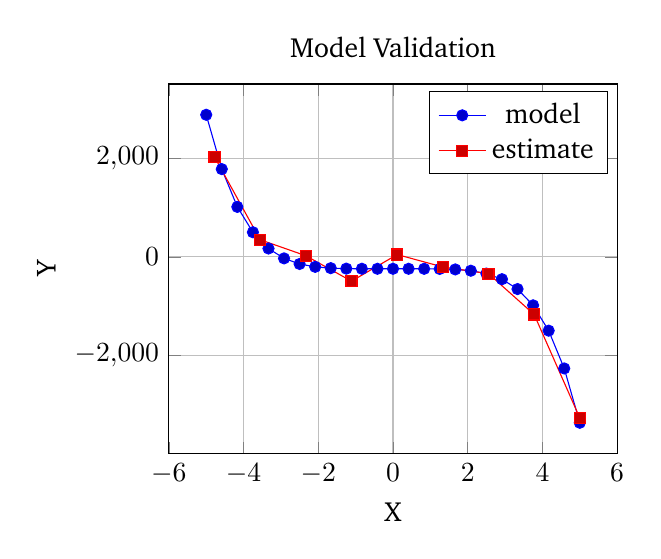
\begin{tikzpicture}
		\begin{axis}[
			width=0.6\textwidth,
			grid=major,
			title={Model Validation},
			xlabel={X},
			ylabel={Y}
		]
			
		\addplot {-x^5 - 242};
		\addlegendentry{model}
	
		\addplot coordinates {
			(-4.77778,2027.60977)
			(-3.55556,347.84069)
			(-2.33333,22.58953)
			(-1.11111,-493.50066)
			(0.11111,46.66082)
			(1.33333,-205.56286)
			(2.55556,-341.40638)
			(3.77778,-1169.24780)
			(5.00000,-3269.56775)
		};
		\addlegendentry{estimate}
		\end{axis}
	\end{tikzpicture}
	\end{figure}
}

\subsection{Frame Numbers}
\frame{
	\frametitle{Frame number instead of page number}
	\setbeamercovered{transparent}
	\begin{itemize}
		\item<1-> Watch the frame number.
		\item<2-> It doesn't change!
	\end{itemize}
}

{
\setbeamercolor{background canvas}{bg=black} % Background color
	\frame[dtuwhitelogo]{
		\frametitle{Hello Blackness}
		Here is another frame style!
	}
}

\section{Final Remarks}

\subsection{Fonts}
\frame{
	\frametitle{Fonts}
	\begin{itemize}
		\item You can set whatever font you like in the preamble. E.g.:
		\begin{itemize}
			\item \texttt{\textbackslash usepackage\{lmodern\} \% Latin Modern}
			\item \texttt{\textbackslash usepackage\{helvet\} \% Helvetica}
			\item \texttt{\textbackslash usepackage\{verdana\} \% Verdana}
			\item \texttt{\textbackslash usepackage\{newtx, newtxmath\} \% Times (text and math)}
		\end{itemize}
		
		\item DTU recommends Verdana but this font type is not available by default on all operating systems:
		\begin{itemize}
			\item Windows: include the \texttt{verdana} package in the preamble and MiKTeX will do the rest;
			\item Linux and OS X: before including the \texttt{verdana} package in your preamble, run the \texttt{install\_fonts.sh} script from our package.
		\end{itemize}
	\end{itemize}        
}

%================================================
%===  Define the contact details
\newcommand\contactTable{ %
  \begin{tabular}{lr}
    \multicolumn{2}{l}{Your Name} \\ 
    \multicolumn{2}{l}{\LaTeX\ Support Group, Technical University of Denmark (DTU)} \\ \midrule
    Building 308, Room 119    & latex-support@student.dtu.dk. \\
    2800 Kgs. Lyngby, Denmark & +45 4525 phone \\
    http://www.latex.dtu.dk   & +45 4525 fax
  \end{tabular}
}%

\frame[dtuwhitelogo, bgfilename=dtu_bg_fiber]{
  \begin{tikzpicture}[remember picture,overlay]
    \node[fill=black, fill opacity=0.9, 
          text=white, text opacity=1.0,
          rounded corners=5pt, 
          font=\scriptsize] at (current page.center) {\contactTable};
  \end{tikzpicture}
}

\frame[dtuwhitelogo, bgfilename=dtu_bg_nano]{
  \begin{tikzpicture}[remember picture,overlay]
    \node[fill=black, fill opacity=0.9, 
          text=white, text opacity=1.0,
          rounded corners=5pt, 
          font=\scriptsize] at (current page.center) {\contactTable};
  \end{tikzpicture}
}

\frame[dtuwhitelogo, bgfilename=dtu_bg_pink]{
  \begin{tikzpicture}[remember picture,overlay]
    \node[fill=white, fill opacity=0.8, 
          text=black, text opacity=1.0,
          rounded corners=5pt, 
          font=\scriptsize] at (current page.center) {\contactTable};
  \end{tikzpicture}
}

\frame{
	\frametitle{Contact}
	
	\begin{center}
		File bugs and feature requests at \url{http://gitlab.cc.dtu.dk/latex/dtutemplates/issues}
	\end{center}
}

\frame[allowframebreaks]{
	\frametitle{Release History}
	\begin{block}{v1.12}
		\begin{itemize}
			\item Frame number instead of page number.
		\end{itemize}
	\end{block}
	\begin{block}{v1.11}
		\begin{itemize}
			\item Long titles are displayed correctly in the footer;
			\item Department logos have the correct RGB color;
			\item The aspect ratio of the slides can be changed using beamer options.
		\end{itemize}
	\end{block}
	\begin{block}{v1.1}
		\begin{itemize}
			\item Fonts options;
			\item Poster template;
			\item Frame backgrounds;
			\item Black frames with white logo;
			\item Address boxes.
		\end{itemize}
	\end{block}
	\begin{block}{v1.03}
		\begin{itemize}
			\item New logos for \texttt{vindenergi} and \texttt{kemiteknik}.
		\end{itemize}
	\end{block}
	\begin{block}{v1.02}
		\begin{itemize}
			\item Date format is now customizable.
		\end{itemize}
	\end{block}
	\begin{block}{v1.01}
		\begin{itemize}
			\item \texttt{dtuletter} template included;
			\item Package name changed to \texttt{dtutemplates}.
		\end{itemize}
	\end{block}
}
\end{document}